\chapter{Burrows-Wheeler-Transformation}

Die \term{Burrows-Wheeler-Transformation}\index{Burrows-Wheeler-Transformation} erzeugt eine sinnvolle Permutation des eingegebenen Strings; sie gruppiert Zeichen mit ähnlichem Kontext nahe beieinander. Die Struktur der Permutation beinhaltet alle Informationen, die benötigt werden, um eine Rücktransformation durchzuführen, es sind also keine Zusatzinformationen nötig. Hin- und Rücktransformation geht in \( O(n) \). Sie wird hauptsächlich zur Vorverarbeitung statischer Texte genutzt, um sie komprimieren, indizieren und in ihnen suchen zu können.

\section{Konstruktion}

Sei \( T = \texttt{lalalangng\$} \) der gegebene String (mit angehängtem \$-Zeichen), \( n = \left\vert T \right\vert \) und \( T^{(i)} \) die \( i \)-te Permutation von \( T \) (durch \( i \) mal den vordersten Buchstaben nehmen und hinten anhängen). Man erhält die Burrows-Wheeler-Transformation von \( T \) so:

\begin{enumerate}
  \item Schreibe \( T^{(1)} \) bis \( T^{(n)} \) untereinander.
  \item Sortiere \( T^{(1)} \) bis \( T^{(n)} \).
  \item Die letzte Spalte ist \( T^{\text{BWT}} \) (\( = L \)), die Burrows-Wheeler-Transformation von \( T \).
\end{enumerate}

\begin{figure}[H]
  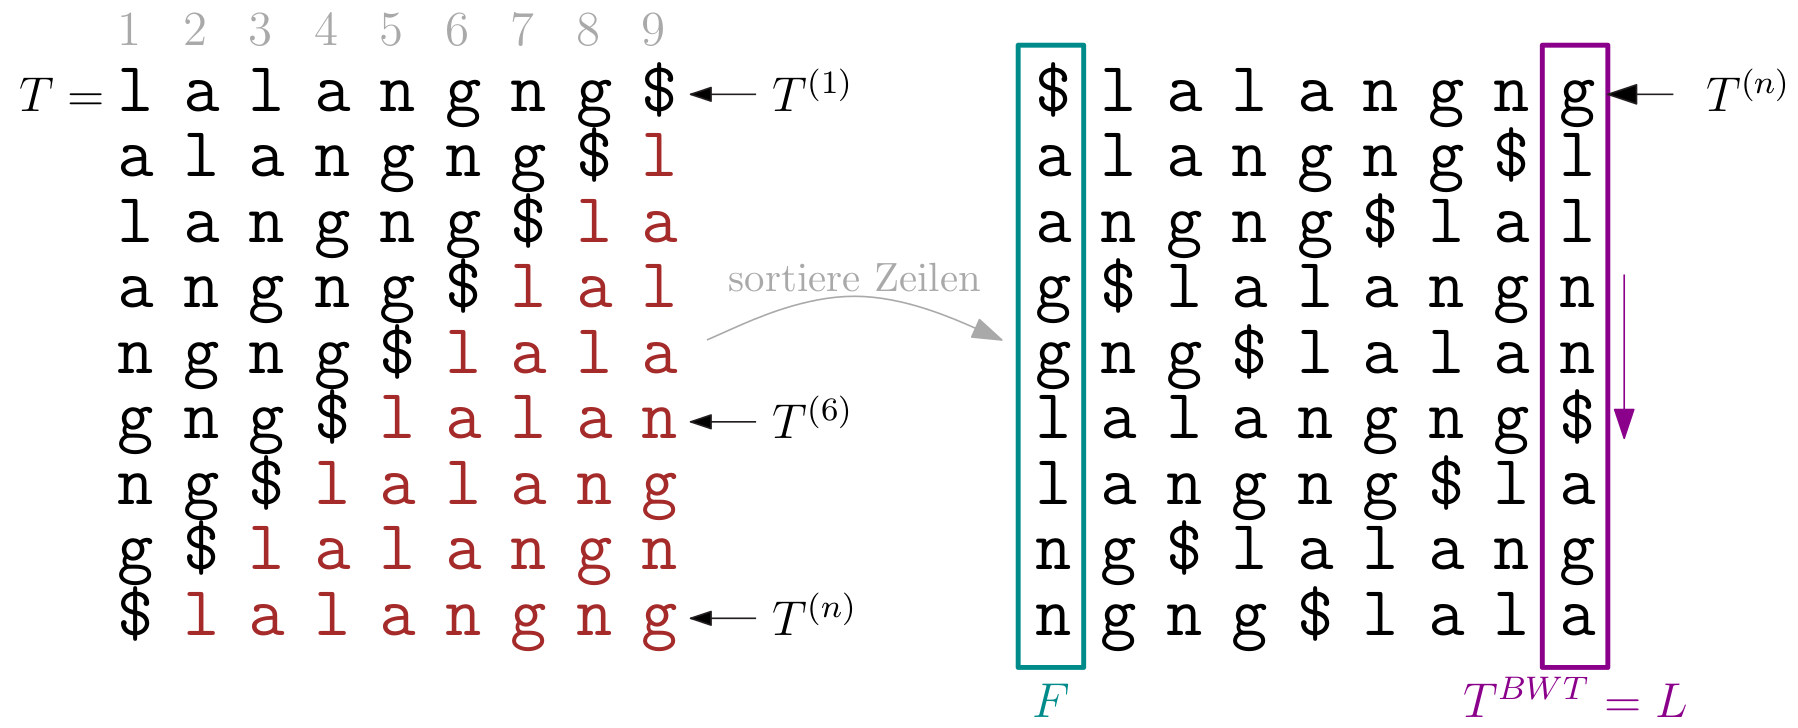
\includegraphics[width=0.7\textwidth]{BWT}
  \caption{Konstruktion der Burrows-Wheler-Transformation von \( T = \texttt{lalalangng\$}  \), \( T^{\text{BWT}} = \texttt{gllnn\$ aga} \). Da \( T^{\text{BWT}} \) die letzte Spalte ist schreibt man oft auch \( L \) stattdessen. Die erste Spalte wird auch \( F \) genannt}
\end{figure}

Naiv benötigt die Berechnung von \( T^{\text{BWT}} \) \( O(n^2 + n\log n) \) Schritte. Die Berechnungszeit lässt sich aber auf \( O(n) \) reduzieren.

\section{Beobachtungen}

Folgende Eigenschaften lassen sich feststellen:

\begin{itemize}
  \item Die Zeilen der oben konstruierten Matrix enthalten die sortierten Suffixe von \( T \) (vom Zeilenstart bis \$ gehend).
  \item Die Zeichen der letzten Spalte (also \( T^{\text{BWT}} \)) sind also die Zeichen, die vor dem zu ihrer Zeile gehörenden Suffix stehen. Formaler ist \( T^{\text{BWT}}[i] \) das Zeichen vor dem \( i \)-ten Suffix in \( T \):
  \begin{equation*}
    T^{\text{BWT}}[i] = L[i] = T[\text{SA}[i]-1] = T^{(\text{SA}[i])}[n]
  \end{equation*}
  Da wir mithilfe des \hyperref[sec:SALinear]{DC3-Algorithmus} das Suffix-Array in Linearzeit berechnen können, können wir auch die Burrows-Wheeler-Transformation in Linearzeit bestimmen.
\end{itemize}

\section{Rücktransformation}

\begin{minipage}{0.8\textwidth}
  Wir können aus einer vorliegenden \( T^{\text{BWT}} \) einfach \( F \) --- also die erste Spalte der Matrix --- konstruieren, indem wir die Buchstaben von \( T^{\text{BWT}} \) sortieren. Hängen wir nun \( T^{\text{BWT}} \) und \( F \) hintereinander, so haben wir bereits Buchstabenpaare, die so auch in \( T \) auftreten. Sortieren wir nun die beiden Spalten (also die Buchstabenpaare) lexikographisch, so erhalten wir die auf \( F \) folgende Spalte. Durch diesen Prozess lässt sich die gesamte Matrix und somit \( T \) rekonstruieren.
\end{minipage}
\hfill
\begin{minipage}{0.15\textwidth}
  \begin{figure}[H]
    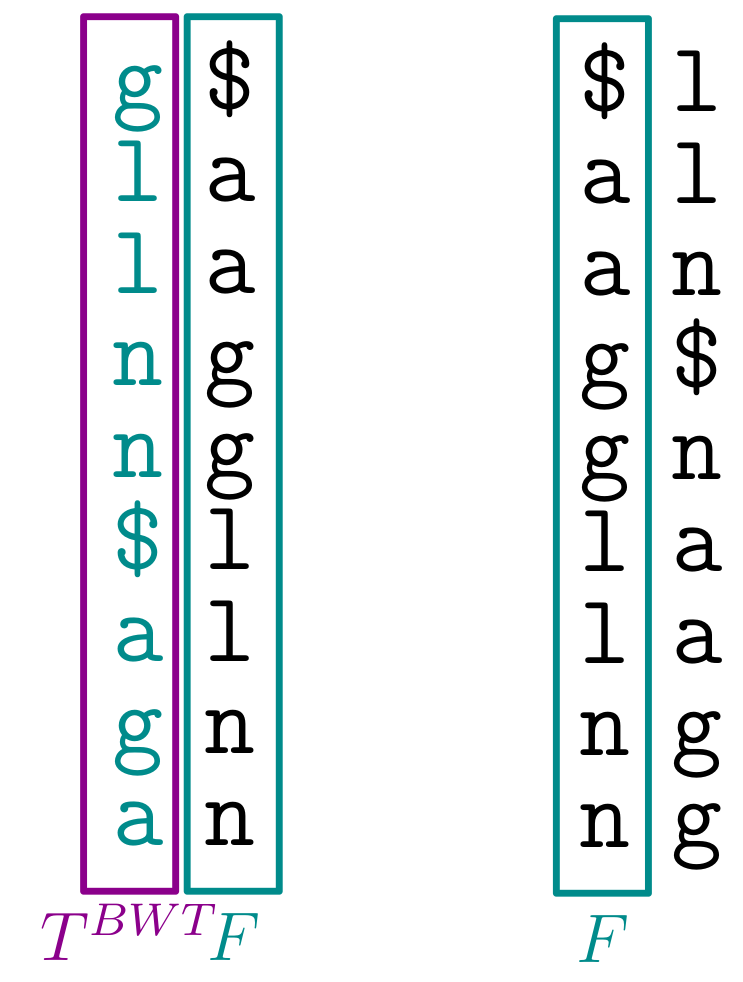
\includegraphics[width=\textwidth]{BWTSorting}
  \end{figure}
\end{minipage}

\clearpage

Diese Art der Rücktransformation benötigt \( O(n^2\log n) \) Schritte. Im Folgenden werden wir die Rücktransformation auf Linearzeit reduzieren. Dazu benötigen wir \term{Last-to-front mapping}\index{Last-to-front mapping}:
\begin{equation*}
  \text{LF}[i] \coloneqq \text{ Position in } L\text{, an der Vorgänger von } L[i] \text{ steht}
\end{equation*}

\begin{minipage}{.65\textwidth}
  Da die Spalten der BWT-Matrix zyklisch sind, ist der Vorgänger von \( L[i] \) derjenige Buchstabe, der in \( F[i] \) steht, also
  \begin{equation*}
    \text{LF}[i] = \text{Position, an der } L[i] \text{ in } F \text{ steht}
  \end{equation*}
\end{minipage}
\hfill
\begin{minipage}{.3\textwidth}
  \begin{figure}[H]
    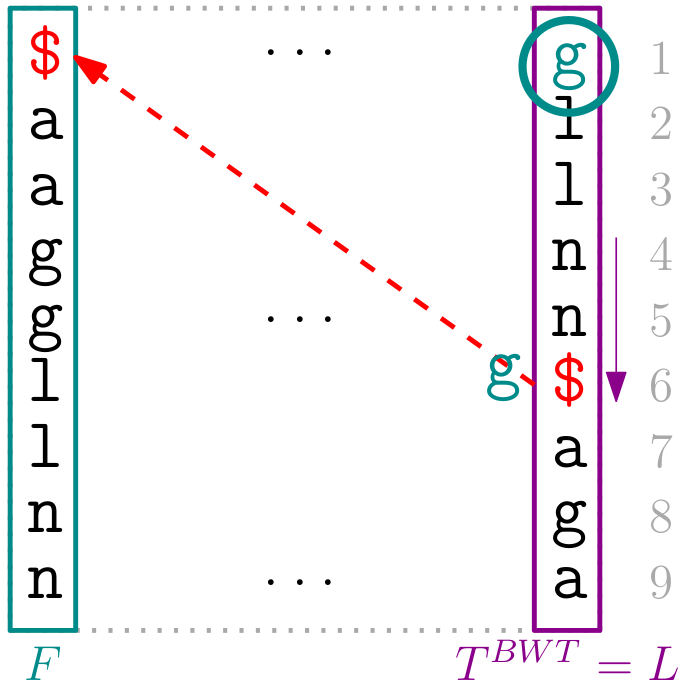
\includegraphics[width=\textwidth]{BWTLF}
    \caption{Gesucht ist der Vorgänger von \texttt{\$}. Stellen wir uns \( T^{\text{BWT}} \) ein zweites Mal links von \( F \) vor, so sehen wir, dass es \texttt{g} ist}
  \end{figure}
\end{minipage}

Wir erhalten folgenden Zusammenhang:
\begin{equation*}
  \text{LF}[i] = j \Leftrightarrow T^{(\text{SA}[j])} = {\left( T^{(\text{SA}[i])} \right)}^{(n)}\text{.}
\end{equation*}

\subsection{Weitere Überlegungen zur Rücktransformation}

Wir können desweiteren folgende Beobachtungen an \( T^{\text{BWT}} \) machen:

\begin{minipage}{.6\textwidth}
  \begin{itemize}
    \item Gleiche Zeichen haben gleiche Reihenfolge in \( F \) und \( L \).
    \item Falls \( L[i] = L[j] \) für \( i < j \), dann ist \( \text{LF}[i] < \text{LF}[j] \).
  \end{itemize}
  Grund dafür ist, dass die Zeilen der BWT-Matrix lexikographisch sortiert sind.
\end{minipage}
\hfill
\begin{minipage}{.35\textwidth}
  \begin{figure}[H]
    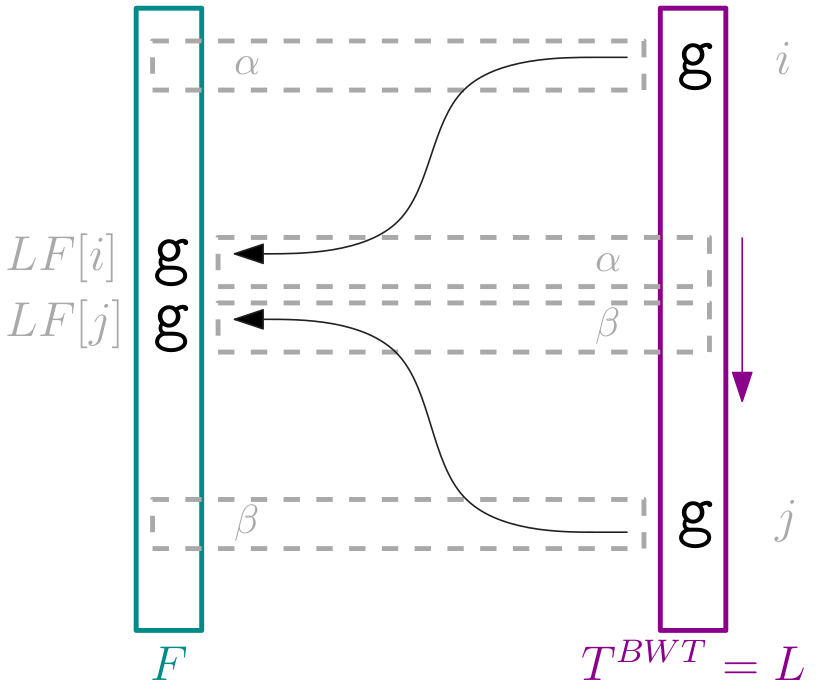
\includegraphics[width=\textwidth]{BWTBack}
    \caption{Präfixe \( \alpha \) und \( \beta \) und wie sie in der Matrix vorkommen}
  \end{figure}
\end{minipage}

Wir können also \( LF \) rein aus \( T^{\text{BWT}} \) berechnen. Dazu brauchen wir nur zwei Hilfsfunktionen:

\begin{itemize}
  \item \( C(a) \coloneqq \# \) Zeichen \( < a \)
  \item \( \text{occ}[i] \coloneqq \# \) Zeichen \( = L[i] \) in \( L[1\dots i] \)
\end{itemize}

Nun können wir \( \text{LF}[i] \) darstellen als
\begin{equation*}
  \text{LF}[i] = C(L[i]) + \text{occ}[i]
\end{equation*}
und können somit \( \text{LF} \) in \( O(n) \) berechnen, da sich \( C \) und \( \text{occ} \) in Linearzeit berechnen lassen.

\subsection{Implementierung}

Zuerst berechnen wir LF. Hier sieht die Implementierung so aus:

\begin{enumerate}
  \item Initialisiere occ und \( h \). \( h \) sei ein Array, das zählt, wie oft ein bestimmter Buchstabe vorkommt, damit wir nachher \( C \) gescheit berechnen können.
  \item Laufe durch \( L = T^{\text{BWT}} \) (\( i = 1 \dots n \))
  \begin{itemize}
    \item \( h(L[i]) \)++
    \item \( \text{occ}(L[i]) = h(L[i]) \)
  \end{itemize}
  \item Konstruiere \( C \) aus \( h \): \( C(\texttt{\$}) = 0 \), \( C(\alpha) = C(\alpha - 1) + h(\alpha - 1) \) (\( \alpha \) ist ein Buchstabe, \( \alpha - 1 \) sein Vorgänger)
  \item \( \text{LF}[i] = C(L[i]) + \text{occ}[i] \)
\end{enumerate}

\begin{figure}[H]
  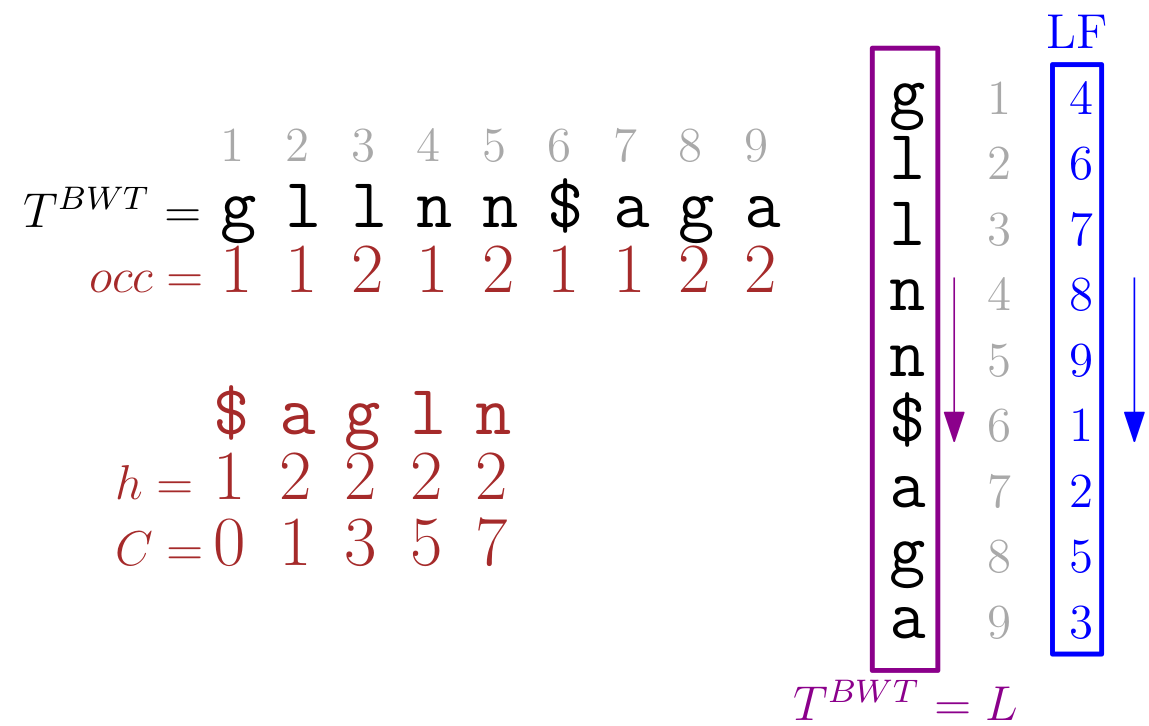
\includegraphics[width=0.6\textwidth]{BWTBackLinear}
  \caption{Beispiel des Algorithmus zur Berechnung von LF nach Durchführung}
\end{figure}

\begin{minipage}{.8\textwidth}
  Nun kann \( T \) von rechts nach links berechnet werden:
  \begin{enumerate}
    \item \( T[n] = \texttt{\$} \Rightarrow \text{LF}[\cdot] = 1 \). Das ist unabhängig von \( T \) so.
    \item \( L[1] = \texttt{g} \Rightarrow T[n-1] = \texttt{g} \Rightarrow \text{LF}[1] = 4 \)
    \item \( L[4] = \texttt{n} \Rightarrow T[n-2] = \texttt{n} \Rightarrow \cdots \)
  \end{enumerate}
  Also geht auch die Rücktransformation in \( O(n) \).
\end{minipage}
\hfill
\begin{minipage}{.15\textwidth}
  \begin{figure}[H]
    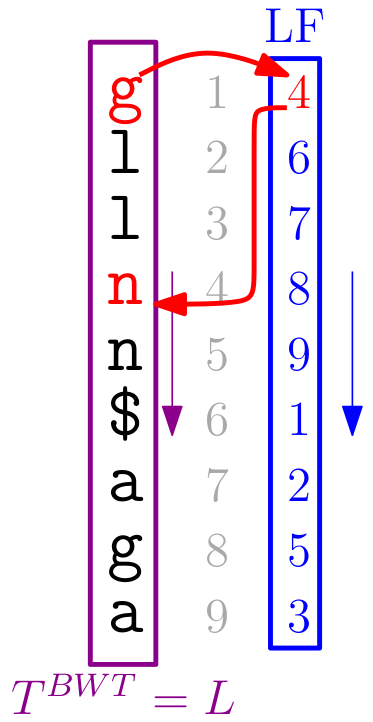
\includegraphics[width=\textwidth]{BWTBackResult}
  \end{figure}
\end{minipage}

\section{Was bringt die BWT?}

Die Vorteile der Burrows-Wheeler-Transformation sind nicht direkt erkennbar --- sie nutzt dieselben Zeichen wie \( T \) und benötigt den gleichen Platz.

Allerdings wird die \emph{Komprimierung stark vereinfacht}, weil Zeichen mit ähnlichem Kontext gruppiert werden. Besonders gut funktioniert sie auf Texten mit vielen gleichen Substrings, wie beispielsweise einem englischen Fließtext. Zur Vereinfachung von \emph{Indexierung} und \emph{Suche} steuert sie auch bei, weil Vorgänger von Suffixen einfach bestimmt werden können.

Im Folgenden werden wir uns die Burrows-Wheeler-Transformation im Kontext von \emph{Kompression} und \emph{Suche} anschauen.

\section{Kompression}

Wir schauen uns zwei Kompressionsmöglichkeiten an: die \emph{move to front}-Kodierung und die Huffman-Kodierung

\subsection{MTF-Kodierung}

Idee der \term{MTF-Kodierung}\index{Kodierung!MTF} ist es, lokale Redundanz zu nutzen und so kleine Zahlen für gleiche Zeichen, die nahe beieinander liegen, zu verwenden. Die Umsetzung funktioniert so:

\begin{enumerate}
  \item Initialisiere \( Y \) mit Alphabet von \( T^{\text{BWT}} \).
  \item Durchlaufe \( T^{\text{BWT}} \) (\( i = 1,\dots,n \))
  \begin{itemize}
    \item Generiere \( R[1,\dots,n] \), wobei \( R[i] \) die Position von \( T^{\text{BWT}}[i] \) in \( Y \) codiert.
    \item Schiebe \( T^{\text{BWT}}[i] \) an den Anfang von \( Y \).
  \end{itemize}
\end{enumerate}

\begin{figure}[H]
  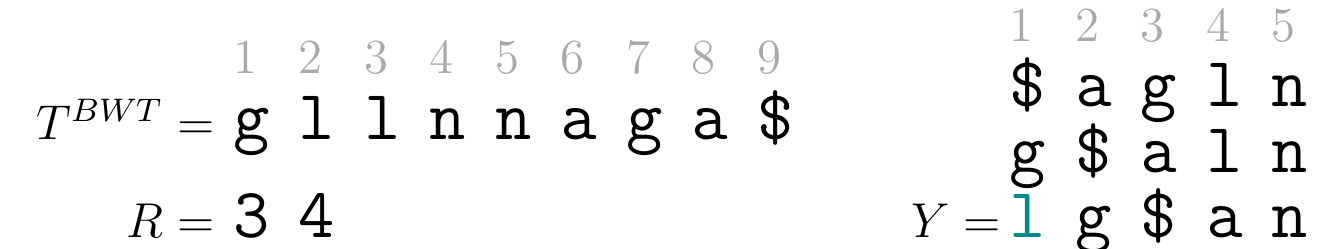
\includegraphics[width=0.8\textwidth]{MTF}
  \caption{Es wurde hier gerade die \texttt{4} eingefügt und deswegen \texttt{l} in \( Y \) nach vorne genommen. Als nächstes muss \texttt{l} codiert (\( \cong \texttt{1} \)) und \( Y \) anschließend nicht verändert werden, weil \texttt{l} ja eh schon ganz vorne steht}
\end{figure}

\clearpage

\subsection{Huffman-Kodierung}

Die \term{Huffman-Kodierung}\index{Kodierung!Huffman} erzeugt präfixfreie Codes variabler Länge. Der Ablauf ist:

\begin{enumerate}
  \item Notiere vorkommende Symbole und ihre jeweiligen Häufigkeiten. Sie sind die Blätter des (binären) Huffman-Baumes.
  \item Verknüpfe die zwei seltenstem Knoten in einem neuen Knoten. Die Häufigkeit des neuen Knotens ist die Summe der Häufigkeiten seiner Kinder. Dies erfolgt nun iterativ.
  \item Die Wurzel hat relative Häufigkeit \( 1 \) (bzw.\ absolute Häufigkeit \( \left\vert T \right\vert \)).
  \item Beschrifte die Kanten zwischen einem Knoten und seinen beiden Kindern mit \( 0 \) und \( 1 \). Der Pfad von der Wurzel zu einem bestimmten Blatt ergibt den Code des Symbols, zu dem das Blatt gehört.
\end{enumerate}

\begin{figure}[H]
  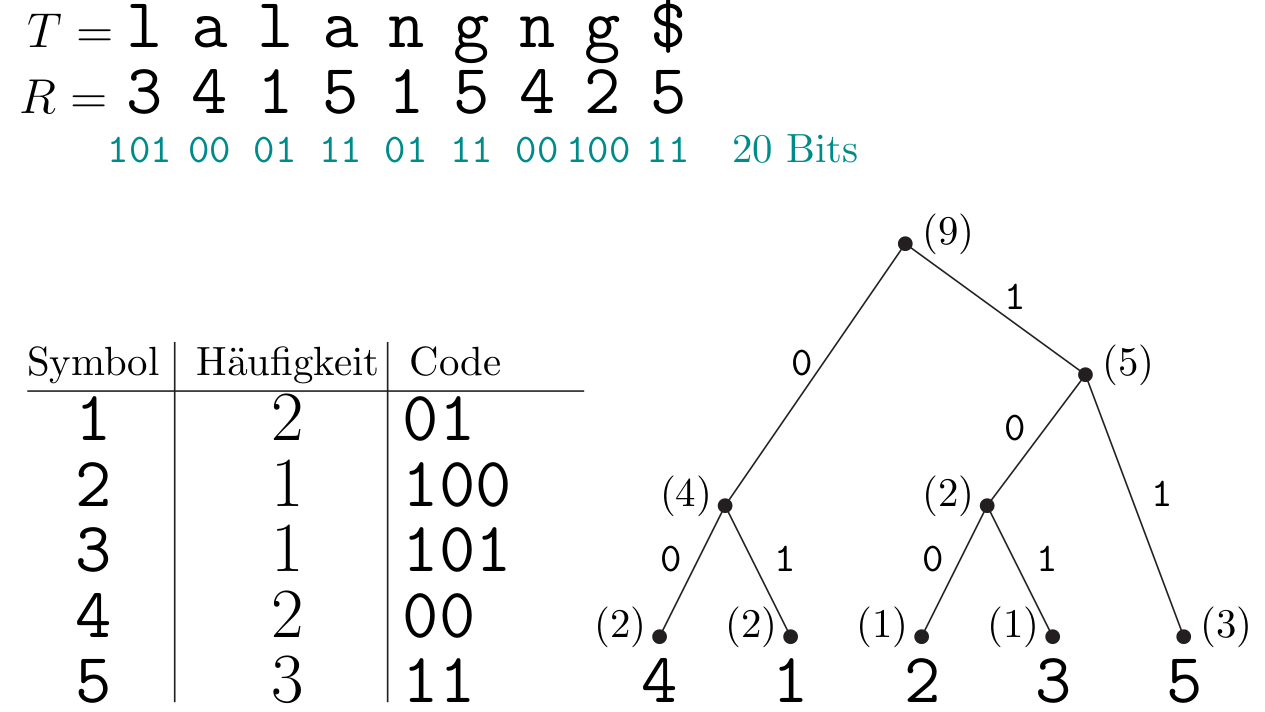
\includegraphics[width=0.6\textwidth]{Huffman}
  \caption{MTF-Kodierung \( R \) von \( T \), die Häufigkeit der in \( R \) vorkommenden Symbole und die mit dem Huffman-Baum erzeugten Codes}
\end{figure}

\section{Suche in der Burrows-Wheeler-Transformation}

Wir möchten nun in \( T^{\text{BWT}} \) nach einem Pattern \( P \) suchen. Hier sei
\begin{align*}
  P &= \texttt{bar} \quad \text{und} \\
  T &= \texttt{abracadabrabarbara\$}\text{.}
\end{align*}
Wir benötigen dazu zwei Hilfsmittel:

\begin{itemize}
  \item Das Array \( C \) beinhalte für jeden eindeutigen Buchstaben in \( t \in T \) die Position des ersten Suffixes im Suffix-Array, das mit \( t \) beginnt.
  \item \( \text{rank}(i,X,\text{ BWT}) \) gibt an, wie oft ein Buchstabe \( X \) in \( \text{BWT}[0,\dots,i-1] \) vorkommt.
\end{itemize}